\newpage
\section{\textbf{Apresentação}}

% ===================== APRESENTAÇÃO =====================

O sistema de proteção de uma rede elétrica tem como função principal detectar condições anormais de operação, em especial os curtos-circuitos, e isolar o mais rapidamente possível apenas a parcela do sistema afetada pelo defeito, preservando a integridade dos equipamentos, a segurança das pessoas e a continuidade do fornecimento às demais cargas \cite{mamede2013}. Para que esse objetivo seja atingido, os dispositivos de proteção devem ser dimensionados e ajustados de forma a atender, simultaneamente, aos requisitos de seletividade, sensibilidade, rapidez e confiabilidade, além de operarem de maneira coordenada entre si \cite{kindermann2005}.

No Campus do Pici da Universidade Federal do Ceará (UFC) são desenvolvidas, além das atividades acadêmicas e administrativas, aulas práticas em laboratórios e diversos projetos de pesquisa e desenvolvimento, muitos dos quais dependem de um suprimento contínuo de energia elétrica \cite{silveira2022}. Nesse contexto, um estudo de proteção bem elaborado é fundamental para garantir que, na ocorrência de uma falta, seja desligado o menor número possível de cargas do campus, e por um tempo mínimo.

Até agosto de 2019, o Campus do Pici era atendido em média tensão (13,8~kV) pelo alimentador PCI01C8 da concessionária local, um alimentador praticamente exclusivo, que atendia apenas duas unidades consumidoras: o próprio Campus do Pici e o Núcleo de Tecnologia Industrial do Ceará (NUTEC) \cite{silveira2019apres}. 


Atualmente, o campus é suprido por uma subestação própria de 69-13,8~kV, denominada SE Campus do Pici, conectada ao Sistema de Distribuição em Alta Tensão (SDAT) da Enel Distribuição Ceará por meio de uma derivação da Linha de Distribuição de Alta Tensão (LDAT) 02L9, que interliga as subestações Pici (SED PCI, barra 7955) e Maguary (SED MGY, barra 9015). A Figura~\ref{fig:unifilar_simplificado} apresenta o diagrama unifilar simplificado do sistema, com os níveis de curto-circuito e as correntes máximas de carga e dos condutores dos alimentadores \cite{sampaio2026roteiro}.

\begin{figure}[htbp]
    \centering
    \caption{Diagrama unifilar simplificado da derivação da LDAT 02L9, da SE Campus do Pici e do Sistema de Distribuição em Média Tensão (SDMT) do campus.}
    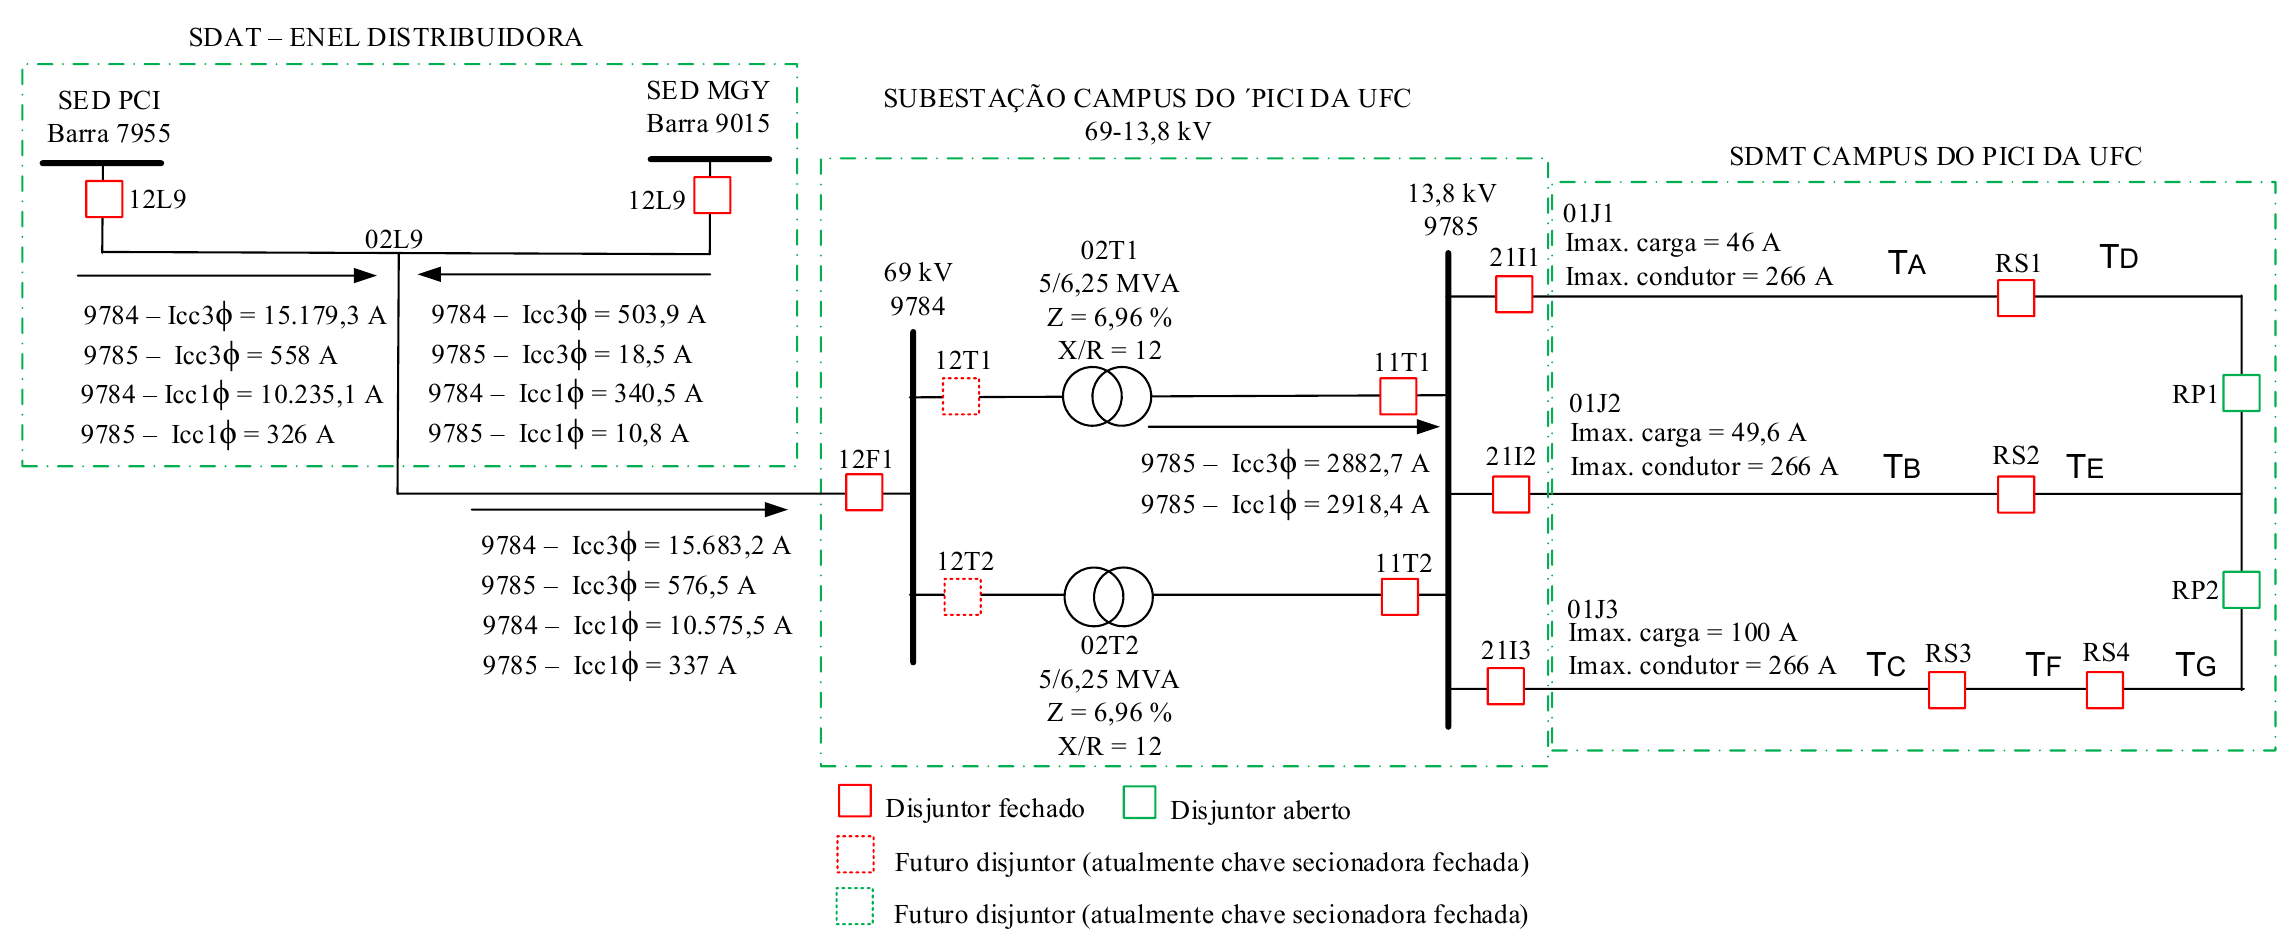
\includegraphics[width=16cm]{Imagens/unifilar_simplificado.png}
    \label{fig:unifilar_simplificado}
    \par\vspace{2pt}
    {\small Fonte: \cite{sampaio2026roteiro}.}
\end{figure}

A subestação é composta por um vão de entrada de linha em 69~kV, protegido pelo disjuntor 12F1, um barramento de 69~kV (barra 9784) e dois transformadores de potência, 02T1 e 02T2, de 5,00/6,25~MVA (ONAN/ONAF), com impedância de 6,96\%, relação $X/R = 12$ e ligação triângulo no primário e estrela aterrada no secundário (Dyn1). Do lado de alta tensão, os transformadores estão atualmente conectados ao barramento por chaves seccionadoras, estando prevista a instalação futura dos disjuntores 12T1 e 12T2. Do lado de média tensão, cada transformador se conecta ao barramento de 13,8~kV (barra 9785) por meio dos disjuntores gerais 11T1 e 11T2. As correntes nominais de cada transformador são de 41,8~A em 69~kV e 209,2~A em 13,8~kV na potência ONAN, e de 52,3~A e 261,5~A, respectivamente, na potência ONAF.

A distribuição em média tensão é feita por três alimentadores radiais, cujas saídas são protegidas pelos disjuntores 21I1, 21I2 e 21I3. Ao longo da rede estão instalados os religadores RS1, RS2, RS3 e RS4, normalmente fechados, que dividem os alimentadores nos trechos $T_A$ a $T_G$. Os pontos de interligação entre alimentadores, RP1 e RP2, operam normalmente abertos, o que confere à rede uma topologia radial com recurso, permitindo a transferência de carga entre alimentadores em situações de contingência. As correntes máximas de carga registradas nos alimentadores 01J1, 01J2 e 01J3 são de 46~A, 49,6~A e 100~A, respectivamente, e os condutores dos troncos possuem capacidade de condução de 266~A \cite{sampaio2026roteiro}.

Os níveis de curto-circuito nas barras da subestação, fornecidos pela concessionária, estão resumidos na Tabela~\ref{tab:niveis_cc}. Nota-se que a contribuição da SED PCI é largamente predominante sobre a da SED MGY. Destaca-se ainda que, por causa da ligação em triângulo do primário dos transformadores, a corrente de falta fase-terra na barra de 13,8~kV é vista no lado de 69~kV com apenas $1/\sqrt{3}$ do seu valor refletido pela relação de transformação, característica que influencia diretamente os ajustes das funções de neutro.

\begin{table}[htbp]
    \centering
    \caption{Níveis de curto-circuito nas barras da SE Campus do Pici, considerando os dois transformadores energizados.}
    \label{tab:niveis_cc}
    \begin{tabular}{lccc}
        \hline
        \textbf{Local da falta} & \textbf{Corrente medida em} & \textbf{$I_{cc3\phi}$ (A)} & \textbf{$I_{cc1\phi}$ (A)} \\
        \hline
        Barra 9784 (69 kV)   & 69 kV (entrada 12F1)   & 15.683,2 & 10.575,5 \\
        Barra 9785 (13,8 kV) & 69 kV (entrada 12F1)   & 576,5    & 337,0    \\
        Barra 9785 (13,8 kV) & 13,8 kV (barramento)   & 2.882,7  & 2.918,4  \\
        \hline
    \end{tabular}
    \par\vspace{2pt}
    {\small Fonte: adaptado de \cite{sampaio2026roteiro}.}
\end{table}

A montante da SE Campus do Pici, a proteção da saída de linha 12L9 da SED PCI é realizada por um relé SEL-411L, cujos ajustes constam na Ordem de Ajuste de Proteção (OAP) nº 046/2018 da concessionária. A função de sobrecorrente temporizada de fase (51) desse relé está ajustada com corrente de \textit{pick-up} de 1.161,6~A (RTC 1200-5), curva IEC muito inversa e dial de tempo 0,12, e a função de neutro (51N) com \textit{pick-up} de 160,8~A, mesma família de curva e dial 0,55 \cite{enel2018oap}. Para um curto-circuito trifásico na barra de 69~kV da subestação do campus, a função 51 da SED PCI opera em cerca de 0,13~s, o que impõe a principal restrição deste estudo: todas as proteções da SE Campus do Pici devem ser ajustadas abaixo das curvas da concessionária, respeitando os intervalos de coordenação estabelecidos.

Nos estudos realizados em 2018, a subestação teve sua proteção implementada com relés SEL-751 na entrada de linha (12F1), nos disjuntores gerais de barra (11T1 e 11T2) e nas saídas de alimentadores (21I1, 21I2 e 21I3), e com um relé SEL-787 na proteção diferencial dos transformadores \cite{ufc2018diagtempo}. A rede elétrica do campus já foi objeto de outros estudos de proteção, entre os quais se destacam o estudo das proteções do sistema elétrico do Campus do Pici realizado na própria disciplina \cite{andrade2016} e o trabalho de conclusão de curso que avaliou o impacto da integração de uma usina fotovoltaica sobre os ajustes da rede, considerando a operação de apenas um transformador \cite{silveira2022}. Diferentemente deste último, o presente projeto considera os dois transformadores energizados simultaneamente, condição que eleva os níveis de curto-circuito no barramento de 13,8~kV.

Diante do exposto, este projeto tem como objetivo realizar o estudo de coordenação e seletividade das proteções da SE Campus do Pici e das saídas dos alimentadores de distribuição em 13,8~kV, seguindo os critérios estabelecidos em \cite{sampaio2026roteiro}. Para isso, o trabalho está organizado da seguinte forma:

\begin{itemize}
    \item[--] apresentação do diagrama unifilar de proteção da subestação, com a identificação das funções de proteção associadas a cada disjuntor;
    \item[--] dimensionamento e especificação dos transformadores de corrente (TCs) pelos métodos da corrente nominal, do curto-circuito, da tensão máxima no secundário e de Stanley E. Zocholl;
    \item[--] estudo de coordenação das proteções de sobrecorrente (funções 50/51, 50/51N, 51NS, 46, 50BF e 79), englobando o cálculo dos ajustes, os coordenogramas, os diagramas de tempo e a elaboração das ordens de ajuste das proteções (OAP);
    \item[--] estudo da proteção diferencial dos transformadores (função 87T), contemplando as ligações e o dimensionamento dos TCs, o cálculo dos ajustes e a curva característica da função diferencial;
    \item[--] conclusões e proposição de melhorias para o sistema de proteção do campus.
\end{itemize}

Os ajustes foram desenvolvidos considerando as margens de coordenação de 0,4~s entre funções temporizadas (51-51 e 51N-51N), 0,2~s para a seletividade lógica, 0,25~s para a falha de disjuntor e 0,1~s para o tempo de operação das funções instantâneas \cite{sampaio2026roteiro}, bem como as características dos relés comerciais adotados \cite{sel2013sel751, abb1997tpu2000r} e os requisitos de IEDs de proteção estabelecidos pela concessionária \cite{enel2022et2178}.